%
% ideale.tex -- Ideale in den ganzen Gaussschen Zahlen
%
% (c) 2021 Prof Dr Andreas Müller, OST Ostschweizer Fachhochschule
%
\documentclass[tikz]{standalone}
\usepackage{amsmath}
\usepackage{times}
\usepackage{txfonts}
\usepackage{pgfplots}
\usepackage{csvsimple}
\usetikzlibrary{arrows,intersections,math}
\begin{document}
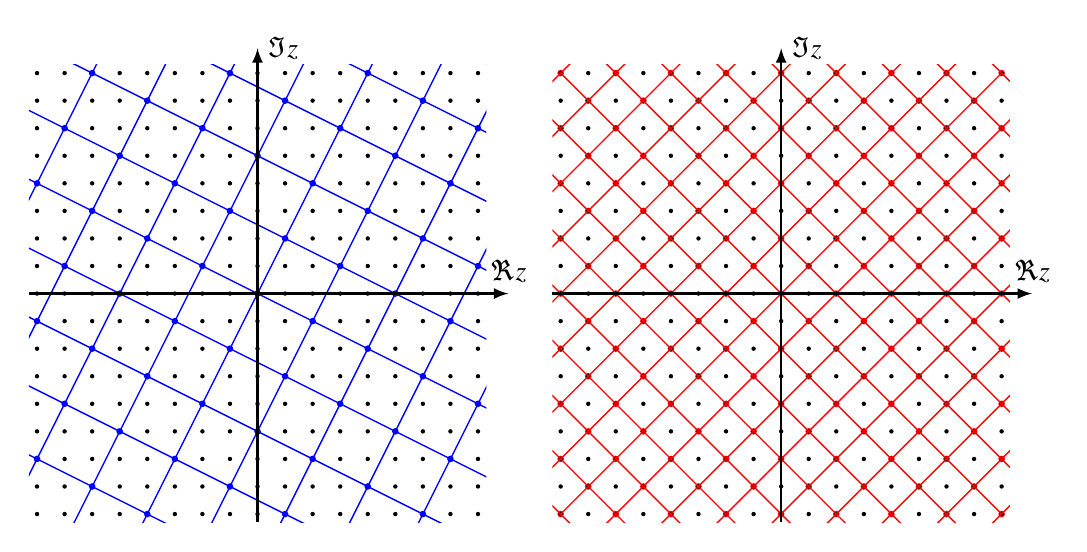
\begin{tikzpicture}[>=latex,thick,scale=0.35]
\begin{scope}[xshift=-9.5cm]
\begin{scope}
\clip (-8.3,-8.3) rectangle (8.3,8.3);
	\foreach \x in {-8,...,8}{
		\foreach \y in {-8,...,8}{
			\fill (\x,\y) circle[radius=0.08];
		}
	}
	\foreach \x in {-8,...,8}{
		\foreach \y in {-8,...,8}{
			\fill[color=blue]
				({\x-2*\y},{2*\x+\y}) circle[radius=0.12];
		}
	}
	\foreach \x in {-8,...,8}{
		\draw[color=blue,line width=0.5pt]
			({\x-2*(-8)},{2*\x+(-8)}) 
			--
			({\x-2*8},{2*\x+8});
	}
	\foreach \y in {-8,...,8}{
		\draw[color=blue,line width=0.5pt]
			({(-8)-2*\y},{2*(-8)+\y}) 
			--
			({8-2*\y},{2*8+\y});
	}
\end{scope}
	\draw[->] (-8.3,0) -- (9.1,0) coordinate[label={$\Re z$}];
	\draw[->] (0,-8.3) -- (0,8.9) coordinate[label={right:$\Im z$}];
\end{scope}

\begin{scope}[xshift=9.5cm]
\begin{scope}
\clip (-8.3,-8.3) rectangle (8.3,8.3);
	\foreach \x in {-8,...,8}{
		\foreach \y in {-8,...,8}{
			\fill[color=red] ({\x-\y},{\x+\y}) circle[radius=0.12];
		}
	}
	\foreach \x in {-8,...,8}{
		\foreach \y in {-8,...,8}{
			\fill (\x,\y) circle[radius=0.08];
		}
	}
	\foreach \x in {-8,...,8}{
		\draw[color=red,line width=0.5pt]
			({\x+8},{\x-8}) -- ({\x-8},{\x+8});
		\draw[color=red,line width=0.5pt]
			({-8-\x},{-8+\x}) -- ({8-\x},{8+\x});
	}
\end{scope}
	\draw[->] (-8.3,0) -- (9.1,0) coordinate[label={$\Re z$}];
	\draw[->] (0,-8.3) -- (0,8.9) coordinate[label={right:$\Im z$}];
\end{scope}

\end{tikzpicture}
\end{document}

